\documentclass{article}
 \usepackage{pgfplots}
 \usepackage{caption}
 \usepackage{tikz}
 \usetikzlibrary{arrows,backgrounds,patterns,shapes.geometric,arrows.meta}
\begin{document}
\begin{figure}[h]
\centering
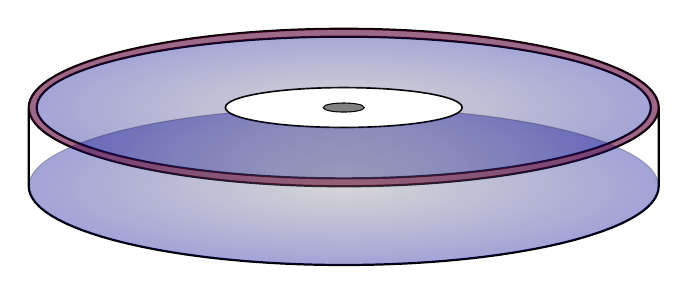
\begin{tikzpicture}

 \draw[thick] (-4,4) -- (-4,3) arc (180:360:4cm and 1cm) -- (4,4) ++ (-4,0) 
 circle (4cm and 1cm);
 \draw[thick]  -- (-1.5,3) arc (180:360:1.5cm and 0.25cm) -- (1.5,4) ++ 
 (-1.5,0) circle (1.5cm and 0.25cm);
 \draw[thick] (4,4) ++ (-4,0) circle (3.9cm and 0.9 cm);
 \filldraw[even odd rule,inner color=white,outer color=blue, opacity = 0.2] 
 (4,4) ++ (-4,0) circle (4cm and 1 cm);
 \filldraw[even odd rule,inner color=white,outer color=blue, opacity = 0.2] 
  (4,4) ++ (-4,-1) circle (4cm and 1 cm);
  \filldraw[even odd rule,inner color=white,outer color=white, opacity = 1]
  (1.5,4) ++ (-1.5,0) circle (1.5cm and 0.25cm);

  \filldraw[even odd rule,inner color=red,outer color=red, opacity = 0.2] 
  (4,4) ++ (-4,0) circle (4cm and 1 cm)
  (4,4) ++ (-4,0) circle (3.9cm and 0.9 cm);
  \draw[thick] (1.5,4) ++ (-1.5,0) circle (0.25cm and 0.05cm);
  \fill[color = gray] 
  (1.5,4) ++ (-1.5,0) circle (0.25cm and 0.05cm);
   \end{tikzpicture}
   
   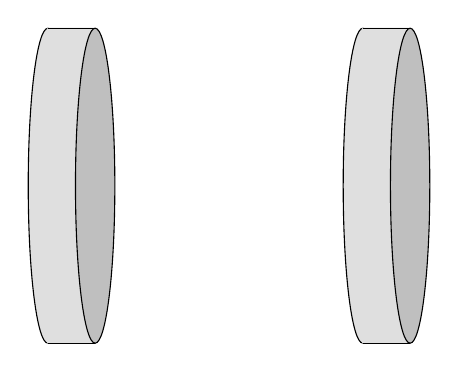
\begin{tikzpicture}
   \filldraw [fill=gray!25,draw=black] (-0.6,0) ellipse (0.25cm and 2cm);
   \filldraw [gray!25] (-0.6,-2) to [bend left=8] (-0.6,2) -- (0,2) to [bend right=8] (0,-2) -- cycle;
   \filldraw [fill=gray!50,draw=black] (0,0) ellipse (0.25cm and 2cm);
   \draw (-0.6,2) --++ (0.6,0);
   \draw (-0.6,-2) --++ (0.6,0);
   
   \begin{scope}[shift=({4,0})]
   \filldraw [fill=gray!25,draw=black] (-0.6,0) ellipse (0.25cm and 2cm);
   \filldraw [gray!25] (-0.6,-2) to [bend left=8] (-0.6,2) -- (0,2) to [bend right=8] (0,-2) -- cycle;
   \filldraw [fill=gray!50,draw=black] (0,0) ellipse (0.25cm and 2cm);
   \draw (-0.6,2) --++ (0.6,0);
   \draw (-0.6,-2) --++ (0.6,0);
   \end{scope}
   
   
   \end{tikzpicture}
  \end{figure}  
    \end{document}